\documentclass{article}
\usepackage{FinalYearProjectReport}

\sloppy

% packages and settings for graphics
\usepackage[pdftex]{graphicx}
\usepackage{booktabs}
\graphicspath{{./}}
\DeclareGraphicsExtensions{.png}
\usepackage[final]{pdfpages}

\setlength\paperheight{297mm}
\setlength\paperwidth{210mm}

\usepackage{avant}
\renewcommand{\familydefault}{\sfdefault}
\frenchspacing

\RequirePackage{hyperref}
\RequirePackage[noabbrev]{cleveref}

\title{Final Report}
\name{Alex \textsc{Andela}, Adil \textsc{Bhayani}, Vaishnavi \textsc{Muppavaram} \& Sakayan \textsc{Sitsabesan}}
\address{Department of Electrical and Computer Engineering\\
University of Auckland, Auckland, New Zealand}

\begin{document}

\begin{titlepage}

\newcommand{\HRule}{\rule{\linewidth}{0.5mm}}

\center
 
%----------------------------------------------------------------------------------------
%	HEADING SECTIONS
%----------------------------------------------------------------------------------------

\textsc{\LARGE University of Auckland}\\[1.5cm]
\textsc{\Large COMPSYS 301: Design: Hardware and Software Systems }\\[0.5cm]
\textsc{\large Autonomous Line Following Robot}\\[0.5cm]

%----------------------------------------------------------------------------------------
%	TITLE SECTION
%----------------------------------------------------------------------------------------

\HRule \\[0.4cm]
{ \huge \bfseries Final Report}\\[0.4cm]
\HRule \\[1.5cm]
 
%----------------------------------------------------------------------------------------
%	AUTHOR SECTION
%----------------------------------------------------------------------------------------

\begin{minipage}{0.4\textwidth}
\begin{flushleft} \large
\emph{Authors:}\\
Alex \textsc{Andela} \newline
Adil \textsc{Bhayani} \newline
Vaishnavi \textsc{Muppavaram} \newline
Sakayan \textsc{Sitsabesan}
\end{flushleft}
\end{minipage}
~
\begin{minipage}{0.4\textwidth}
\begin{flushright} \large
\emph{Supervisors:} \\
Dr. Nitish \textsc{Patel} \\
Dr. Muhammad \textsc{Nadeem} % Supervisor's Name
\end{flushright}
\end{minipage}\\[1cm]

%----------------------------------------------------------------------------------------
%	DATE SECTION
%----------------------------------------------------------------------------------------

{\large \today}\\[2cm]

%----------------------------------------------------------------------------------------
%	LOGO SECTION
%----------------------------------------------------------------------------------------


\includegraphics{uoa.png}\\[1cm]
 
%----------------------------------------------------------------------------------------

\vfill

\vspace*{25em}

{\Large Declaration of Originality}

\hspace{5em}

This report is our own unaided work and was not copied from nor written in collaboration with any other person.

Name: Alex \textsc{Andela}, Adil \textsc{Bhayani}, Vaishnavi \textsc{Muppavaram} \& Sakayan \textsc{Sitsabesan}

\newpage

{\Large Acknowledgments}

\hspace{5em}

We would like to thank our supervisors, Dr. Nitish Patel \& Dr. Muhammad Nadeem, for guiding us throughout the semester with their constant help, supervision and suggestions. We would also like to thank Fung Yang \& Howard Lu for their patience dealing with our numerous issues and changes with the robot hardware. Special mentions need to be made to Joseph Tsoi, Andrew Lai \& John Zhang for their ideas and assistance.

\end{titlepage}

\newpage

\maketitle

%----------------------------------------------------------------------------------------
%	ABSTRACT
%----------------------------------------------------------------------------------------

\begin{abstract}
This project consisted of designing and developing a line following robot that can play a form of the Pacman game. Various analogue and digital design skills were incorporated and developed throughout the duration of this project. The objective was to develop professional engineering skills, including a methodology for both approaching a problem, and for budgeting time, effort and resources. 
\end{abstract}

%----------------------------------------------------------------------------------------
%	INTRODUCTION
%----------------------------------------------------------------------------------------

\section{Design Overview}

This project consists of the design and construction of part of an autonomous line following robot, which is to complete certain benchmarks and pick up "food pellets" dispersed around a given maze. There are two levels of operation. In the first, the objective is to collect food pellets that exist at every coordinate in the maze. The second objective is to collect food pellets at pre-specified coordinates by taking the shortest path.

Pathfinding and control algorithms were vital for the successful functioning of the robot. Various known pathfinding algorithms were explored, before finally deciding on Depth First Search for level one, and A* for level two.  The PID control algorithm was also utilised to ensure that the robot functioned at a set speed, despite its battery voltage.
 
Much of the robot's hardware was prescribed and provided in an assembled state. The sensor circuit required for line detection was the primary aspect of the hardware that needed to be considered as part of this project. The robot was controlled from a Cypress PSoC 5LP, which interfaced with the light sensors, RF, Bluetooth \& Motors to allow the robot to meet its objectives. This report outlines the hardware and software considerations and decisions that were made as part of this project.

%----------------------------------------------------------------------------------------
%	ANALOGUE SECION
%----------------------------------------------------------------------------------------
% Mention considerations and decisions here

\section{Analogue}

The portion of the hardware that needed to be developed as part of this project centred around the collection and processing of vision information. This was done in the form of a surface mounted phototransistor, the TEMT6200. The map is projected down from a ceiling mounted projector, where black lines represent lines and white areas symbolizes the walls. The aim of the analogue portion of this project is to sense the difference between these and convey this information to the PSoC. The following sections outline the considerations and decisions the made by the group while developing the analogue components of this project.

\subsection{Phototransistor output signal}

The phototransistor can be configured in two ways: common emitter or common collector. For this design the common base configuration was not viable as the base of the transistor was unable to be connected to the circuit. In the common collector configuration, the output signal was very flat $(Black: V_{avg} = 2.58V, V_{Pk-Pk} = 0.05V, White: V_{avg} = 2.74V, V_{Pk-Pk} = 0.10V)$ and difficult to differentiate between the black and white lines. On the other hand in the common emitter configuration, there was a sharp difference between the black and white lines $(Black: V_{avg} = 4.09V, V_{Pk-Pk} = 0.09V, White: V_{avg} = 2.84V, V_{Pk-Pk} = 1.54V)$. As a result, a decision was made to use the common emitter configuration for the light sensors.
\subsection{Circuitry}

There were two main concerns in the phototransistor output signal that was to be resolved by the circuitry; these being the removal of the DC offset in the signal, and the filtering of noise. The DC offset needed to be removed as this varied depending on projector brightness in various parts of the map \& external lighting. The projector to be used for this project has a refresh rate of 120Hz, while the ambient light source in the laboratory has a refresh rate of 100Hz. Therefore, a high pass filter with a cut-off less than 120Hz was necessary for this project. In this regard, the group's decision was to implement a RC High Pass filter with a cut-off frequency of 106Hz. This filtered signal was then fed through a non-inverting amplifier with a gain of approximately 20, to further differentiate between black and white projector light readings, and to be used in the next stage of the analogue circuitry. 

The next design aspect that needed to be considered was how the signal would be passed into the PSoC, in digital or analogue form. If the signal were to be passed in as an analogue signal, the PSoC must sample the signal and process this into a binary output (black or white) at a rate fast enough for the robot to accurately follow the line. Alternatively, a hardware Schmitt Trigger could be used on the output signal to create a digital binary output which can be read from the PSoC digital input pins. This solution would process the information into what is relevant to in real time. After much thought and weighing of the pros and cons, a decision was reached to use a Schmitt Trigger and process the signal into a digital signal to be passed into the PSoC.

\subsection{Light sensor array and robot orientation}

The project required a sensor circuit layout that allowed for maximum communication of the robot’s position on the maze, so that the robot can interpret the track and make well-informed decisions on where to move to next. After doing much research into the intricacies of line following robots, it became apparent that a line could be followed with as few as two sensors.

One sensor immediately on either side of the inside of the line is sufficient to track a line and follow it. These two sensors must be placed as far forward as possible so as to make the deviations of the robot more pronounced and easier to detect \& correct. This would result in the robot being able to follow the lines more smoothly and jerk a lot less than if the sensors were near the axis of the wheels. 

To further dampen the oscillations, it was necessary to accurately know how far off the line the robot has deviated. For this purpose, two additional sensors were added on either side of the line slightly behind the front two sensors. These two sensors allowed the robot to calculate how far off the line it had deviated and hence apply the correct correction to return back to the line. 

In this project it was not sufficient for the robot to follow a line. It should additionally be able detect intersections and execute 90$^{\circ}$ turns. For this purpose, two addition sensors were placed at the extreme ends of the board along the front edge of the PCB. These were placed forward so that when an intersection was detected by these sensors, there was enough of a braking distance for the robot to brake in time to turn at the intersection. This was a modification that was made to the sensor array when testing, as the robot displayed that the centre four sensors were not sufficient to accurately track intersections.

\subsection{PCB Design}

An important decision that needed to be made with regards to the PCB design was the use of through-hole mounted (THM) or Surface Mounted Devices (SMD) components.

The use of through hole components would allow for rapid prototyping of the board, with ease of switching out components after assembly. As the component leads run through the board and are soldered over a larger surface area, through-hole mounted circuit boards offer higher reliability and stronger connections. This is very important in cases where there are extreme accelerations, collisions or high temperatures.

Surface mount technology does not require holes to be drilled through the board, are much smaller, can be automatically placed, and can be mounted on both sides of the board. This usually leads to smaller physical area being taken up, higher component density, lower cost, and faster assembly times. 

In this project, higher reliability and extreme environmental conditions were not of major concern. The benefits of surface mount technology allowed for quicker design and assembly time for this project. Hence, after careful consideration the group came decided to use SMD components for the design and assembly of the PCB.

Other considerations for the PCB design included the routing of the pins to the PSoC, whether the H-Bridges would be connected via traces, and the presence of switches for easy operation. The pin assignments to be used for routing the pins to the PSoC were very carefully planned and executed. Much consideration was put into reducing track lengths and making certain that only usable pins were used.

Two bi-polar switches that are easy to operate were used as power on/off switches for the board and localization LEDs. This decision was made as it allowed both the PCB and the localization LEDs to be individually turned on and off. This was important when sharing the maze with other groups' robots without interference. Additionally, two 2-DIP switches were added to enable easy switching between the various modes and configurations of the robot.

Connecting the H-bridges via traces would result in a cleaner design with no rogue wires, but would come at the expense of having more long pins connecting the PCB to the daughterboard, which would cause additional difficulty when assembling the two together. A decision was made to connect via traces as it was realized that the board need not be connected together many times and that this small inconvenience was well worth the much tidier robot connections. The PCB was designed using the `Rooms' feature in Altium Designer to minimize development time for identical circuits, as there was one circuit for each light sensor.

\subsection{Testing and Verification}

Testing, Validation \& Verification of an analogue design are essential components of the development process. As part of this design project, it was ensured that every one of these steps were executed properly. The first stage that took place was verification of the design using LTSpice.

During AC simulation it was found that there had been a calculation mistake with calculating the filter circuit capacitor value. This was promptly corrected. Another issue that arose was the long response time associated with the Schmitt Trigger. This was found to be a result of the unnecessarily large capacitor placed in front of Schmitt trigger for smoothening the input signal. This capacitor was replaced with a capacitor of a slightly lower value to balance response time and correct operation of the circuit.

During the validation stage of the development, the circuit design was tested using a breadboard, and no further complications arose. It was also decided to validate the sensor circuit considerations, by strapping the breadboard onto the robot to see how well it followed the lines. By doing this the conclusion was made that using only two sensors was not sufficient to follow a line, and that additional sensors must also be used. 

During the verification stage of the sensor layout, it was found that the sensor layout only allowed lines to be followed accurately, but did not allow intersections to be accurately detected. Being able to locate intersections were a key part of traversing the Pacman maze, so this was a critical issue that needed to be resolved. This problem was rectified by moving the rear two backup sensors to the front edges of the PCB. These sensors were placed such that they would emit logic HIGH when the robot reached an intersection and not when the robot had deviated from the line.

\subsection{Final Design}

The PCB was designed and assembled using SMD components to minimize board usage and fit all the required components in the given area. The final analogue circuit design used the light sensor phototransistors in the common emitter configuration. This signal was then filtered using a simple RC high pass filter and gain stages followed by a peak detector and Schmitt trigger circuit. This yielded an accurate output of logic HIGH for on the line and logic LOW for off the line.

%----------------------------------------------------------------------------------------
%	DIGITAL SECION
%----------------------------------------------------------------------------------------
% Mention considerations and decisions here

\section{Digital}

The majority of development that took place for the successful completion of this project was digital. This implementation took place using C for execution on the PSoC 5LP. The inputs used to implement the robot line following and maze traversing logic came from RF data, quadrature decoder readings, and light sensor data. 

Alongside the path finding algorithms used in this project, the robot should be able to move to next target location using the shortest path. For level 1 this meant traversing the entire map in the shortest distance, and for level 2, this meant collecting the pre-specified food pellets in the shortest distance between pellets. This section of the report covers the findings and design considerations that were made while these solutions were developed.

\subsection{Path Finding Algorithms}

There were numerous ways to find the shortest path to a particular location in a maze, of these Depth First Search (DFS) and A* algorithms were considered. Both these algorithms were used for pacman level 1 however only A* was used for level 2. 

When attempting to reach the target location, DFS navigated by following a path until the depth of the path was reached, and then traversing backwards until the previous intersection after which it chose the next undiscovered path. For this purpose a maze can be modelled as a tree with nodes in it where each intersection on the maze can be considered a node. This algorithm could have been implemented using recursion or iteration. A few issues with this method included, it did not find the shortest path, if loops existed additional marking was necessary to solve, and most importantly it often lead to suboptimal performance because it did not prioritise direction based on the goal.

On the other hand, the A* algorithm was a much better transversal algorithm in most cases. Given a start and end position, A* prioritised which nodes to discover by using heuristics which estimated how far the node was from the goal. After which the search continued from where it thought was the closest to the goal. The Manhattan heuristic was used in the implementation as it provided the distance between two points on a grid assuming strictly horizontal or vertical movements and the absence of objects.

It was also found that often in multipath mazes where there was more than one path to the destination, finding the shortest path could take longer due to backtracking. In these cases it was usually better to continue on the chosen path than to traverse back a large distance to get the shortest path.

\subsection{Motor Control \& PID}

There were two different ways to design the motor control of the robot. The pins of interest in the H-Bridge used in the design of this robot were the two input pins, an enable pin, two disable pins \& slew rate pin. Of these the slew rate pin must be high for a fast slew rate response of the H bridge. The pin is low by default. It was decided to keep this pin high to set the H bridge in high slew rate mode as there were no obvious disadvantages to this and it meant quicker response times for robot operation.

Any one of the input pins, enable pins or disable pins can be used to modulate the power going to the motors and control the motor speed. At the time of development, the flexibility of this was unbeknownst. Hence, the decision was made to keep the enable and disable pins constant and pulse wave modulate the input pins. This seemed to be the most logical option. Looking back at this now, it can be seen that there are no major advantages to one method over the other.

\subsection{Motion Control \& Line Following}

For the robot to autonomously line follow, there are three sources of information for the robot: RF localization data, quadrature decoder readings, and light sensors. Of these, it was discovered during the course of the project that the RF localization data was very unreliable and very hard to use.

Quadrature decoder readings allowed us to see the distance that the robot's wheels have travelled over a certain time period. This allowed us to track the speed of and distance travelled by the robot. Relying solely on quadrature readings for navigating the maze was considered and explored. It was found that the concave shape of the projector lens resulted in the sizes of a grid being different depending on the part of the maze the robot is in. This resulted in the decision to not use the quadrature readings as the primary source of information for following the lines.

Comparatively, the light sensor data was the most reliable and in the end was the primary source of information used by the robot to make decisions on how to move. As much of the processing of the light sensor data was done in the analogue domain, it was sufficient to just read the pins current voltage level.

Two methods of maze traversal were considered by the group: moving one grid coordinate at a time and moving one intersection at a time. Both methods presented their own challenges and advantages.

Moving one grid at a time allowed more finer control over how the robot traversed the maze and would allow maze solving and robot movements to be interleaved my closely. The main disadvantage with this method was that it was impossible to interpret when grid spaces finish using light sensors, meaning that quadrature sensors and RF data would solely be relied up to ascertain this. Due to the reasons mentioned above, this made this method inviable for the project.

Contrastingly, when moving one intersection at a time, the light sensors are able to very accurately and precisely detect and stop the robot at each intersection. This method also simplified coding as less instructions needed to be made to traverse any particular maze. As the food pellets were to be placed at locations that are not intersections, relying on only this method will always lead to not taking the shortest path. As a result a mixture of these two methods were used with the robot moving intersection to intersection until the final stretch where it moves grid by grid.

\subsection{RF \& Bluetooth}

RF and Bluetooth are two methods of wireless communication that the robot can interface with. The serial RF stream coming from the projector control computer can be received in binary form as a C Struct or a space separated ASCII string. The ASCII string is human readable and easier to work with initially, however the processing time required to convert this into something usable is much greater than for receiving and storing the binary C Struct. The coding required to achieve this is more tedious and repetitive but much easier than the binary method. As a result of weighing both sides, it was decided to use the binary form C Struct method of RF reception.

The Bluetooth module used enabled bi-direction wireless communication between the robot and a computer. This presented numerous opportunities, a few of which were explored in this project. The possibility of Bluetooth boot loading the PSoC was one of the more ambitious ideas that was considered. After setting this up, it was found that it took 45+ seconds to download the program to the PSoC over Bluetooth and it was prone to cut-outs due to signal loss. Due to this, this possibility was not explored any further and was not used in the final project.

Other uses of the Bluetooth module including passing in input arguments for particular modes of operations, outputting status information about the robot and using this as a channel for debugging. These options were well used and were critical to saving a lot of development time and keeping the final project flexible.

\subsection{Data Structures}

There was a large amount of data that was being collected and processed by the robot while in operation. Although primitive data types can be used to store and process this data, this was not ideal for execution or for the programmer. The use of data structures was an essential part of this project to ensure that the data being used was stored in an organized manner, and allowed to be used as efficiently as possible. 

Programming a microcontroller was a primary aspect of the digital design of this project, hence some key design criteria were to keep memory and data usage low. The uses of complex data structures like linked lists and classes were avoided. This was because they added significant overhead that was not seen as worthy. Data structures that were used instead were arrays and structs.

One dimensional and two dimensional arrays were used extensively in the line following algorithms used in this project. They were used to effectively and efficiently store and access the map data, the path the robot has taken, the path the robot should take, where the food pellets are located, etc. Structs were used to receive and access the RF data coming from the project control PC, thereby enabling accurate tracking of robot positioning.

\subsection{Testing and Verification}

The implementation of the two path finding algorithms were first tested using GCC \& GDB to compile and debug the code being worked on. Once this gave satisfactory results, the code was recompiled using the PSoC Creator environment and run and on the PSoC itself. This method of testing \& verification was used as the debugging tools on the PSoC environment were not as easy to use as that provided by GCC \& GDB. The only issue with this process was that sometimes, the program would use more memory than the PSoC had. To ensure this didn't cause any problems, the algorithms were developed with a low memory footprint in mind.

The PID \& motor control part of the code was tested by using the Bluetooth module to send back data from the robot to the computer from the quadrature decoders and RF signal. This data was later plotted and analysed using MATLAB to verify the correct operation of the PID controller. Tuning the PID controller was quite tedious as the tuning values had to be repeatedly changed, and new data collected, before it could be analysed again.

\subsection{Final Design}

Both the A* and DFS algorithms were used in the final design. The A* algorithm (\Cref{fig:astar}) was used in level two to find the shortest path to the next food pellet. The DFS algorithm (\Cref{fig:dfs}) was used in level one, with aspects of A* integrated into it to transverse the entire map in an efficient manner. The PID controller was used in the final implementation to ensure the motor was travelling at the desired speed with minimal oscillations. Digital input pins on the PSoC were used as the primary method of deducing the robot's position on the map by, reading input from the light sensor circuits.

%----------------------------------------------------------------------------------------
%	CONCLUSIONS
%----------------------------------------------------------------------------------------

\section{Conclusions}

As part of this project an autonomous line following robot that can play a form of pacman was designed and developed. The robot was able to traverse the maze, following the lines and collect the required food pellets in the shortest time/distance. A simple analogue circuit was developed to process the light sensor readings into digital signals for feeding into the PSoC. This was built using SMD components on a PCB design that took advantage of the `rooms' feature in Altium Designer. An effective sensor layout was devised such that the robot can follow a line with minimal deviations and accurately detect intersections. A* and DFS path finding algorithms were both used to effectively to best meet the reqirements of each level. A PID contoller was used to ensure the motors of the robot were used to effectively. Through undertaking this project, the group members were able to significantly develop their professional engineering skills. In particular, the communications skills, both written and oral, of the group members were improved, as well as gaining more experience of working in a team to solve a problem. A methodology for both approaching a problem, and for budgeting time, effort and resources was also developed as part of this project.

\clearpage

\section{Contributions}

\begin{table}[h]
\centering
\label{my-label}
\begin{tabular}{@{}l|cccc@{}}
\toprule
Task                          & \multicolumn{1}{l}{Alex Andela} & \multicolumn{1}{l}{Adil Bhayani} & \multicolumn{1}{l}{Vaishnavi Muppavaram} & \multicolumn{1}{l}{Sakayan Sitsabesan} \\ \midrule
Analogue Design               & 40\%                            & 0\%                              & 50\%                                     & 10\%                                   \\
Analogue Testing              & 50\%                            & 0\%                              & 40\%                                     & 10\%                                   \\
Hardware Assembly             & 0\%                             & 10\%                             & 30\%                                     & 60\%                                   \\
PID Control                   & 0\%                             & 40\%                             & 0\%                                      & 60\%                                   \\
Matlab Algorithm              & 0\%                             & 100\%                            & 0\%                                      & 0\%                                    \\
Pacman Algorithms             & 30\%                            & 40\%                             & 30\%                                     & 0\%                                    \\
Benchmark Tasks               & 20\%                            & 30\%                             & 20\%                                     & 30\%                                   \\
Project Archiving             & 55\%                            & 5\%                              & 25\%                                     & 15\%                                   \\
Integration & 30\%                            & 0\%                              & 30\%                                     & 40\%                                   			\\
Report				&25\%			&25\%				&25\%						&25\%			\\ \bottomrule
\end{tabular}
\end{table}

%----------------------------------------------------------------------------------------
%	APPENDICES
%----------------------------------------------------------------------------------------

\clearpage

\section{Appendix A}

\begin{figure}[!h]
\centerline{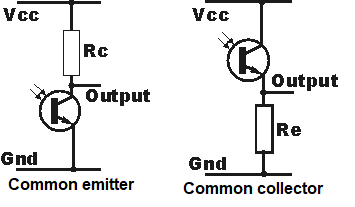
\includegraphics[width=0.5\textwidth]{transistor-config}}
\caption{Transistor Configuration}
\label{fig:transconfig}
\end{figure}

\begin{figure}[!h]
\centerline{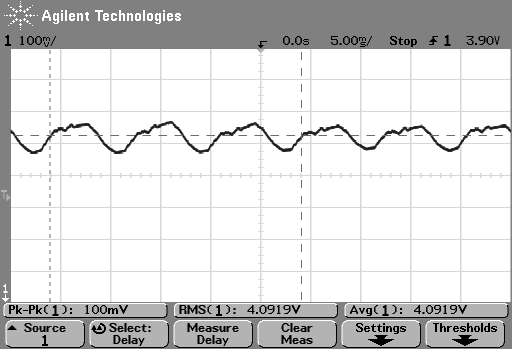
\includegraphics[width=0.5\textwidth]{Waveform-BlackLine}}
\caption{Sensor Output Waveform for Black}
\label{fig:waveblack}
\end{figure}

\begin{figure}[!h]
\centerline{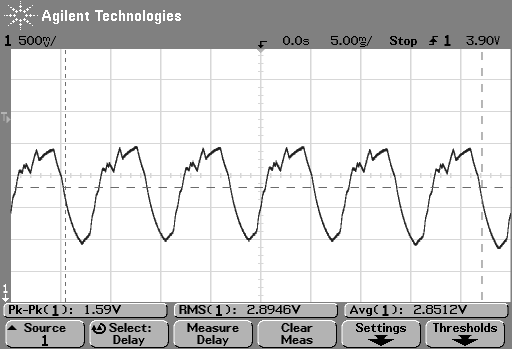
\includegraphics[width=0.5\textwidth]{Waveform-White}}
\caption{Sensor Output Waveform for White}
\label{fig:wavewhite}
\end{figure}

\begin{figure}[!h]
\centerline{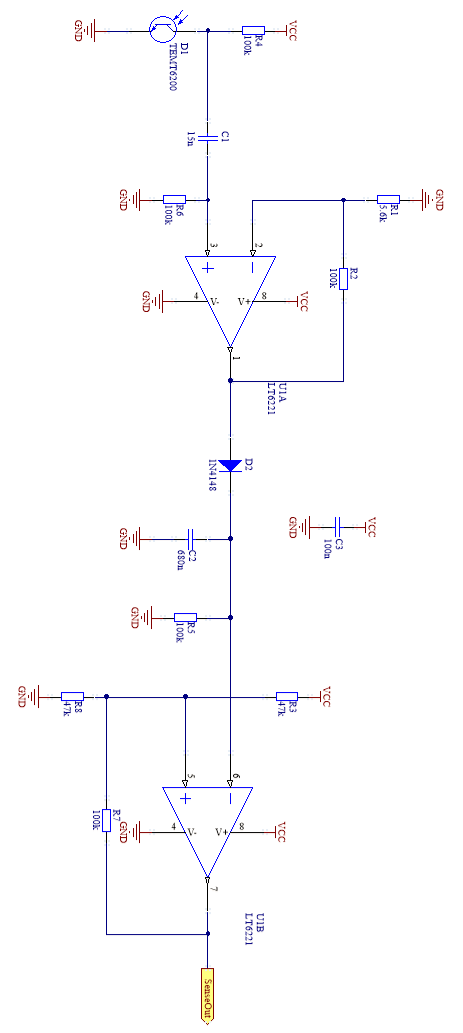
\includegraphics[width=0.5\textwidth]{circuit}}
\caption{Analogue Circuit Diagram}
\label{fig:circuit}
\end{figure}

\begin{figure}[!h]
\centerline{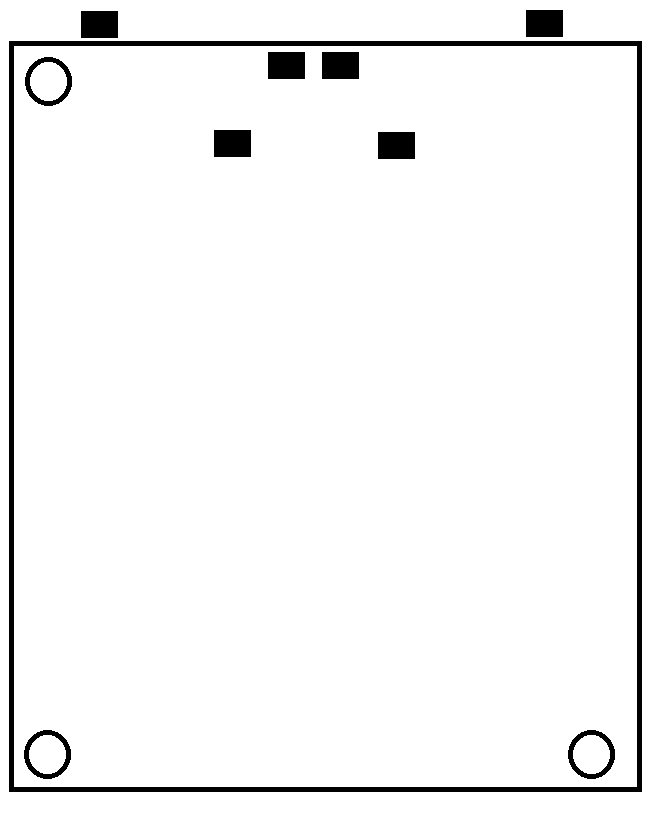
\includegraphics[width=0.5\textwidth]{sensor_layout}}
\caption{Sensor Layout}
\label{fig:senslay}
\end{figure}

\begin{figure}[!h]
\centerline{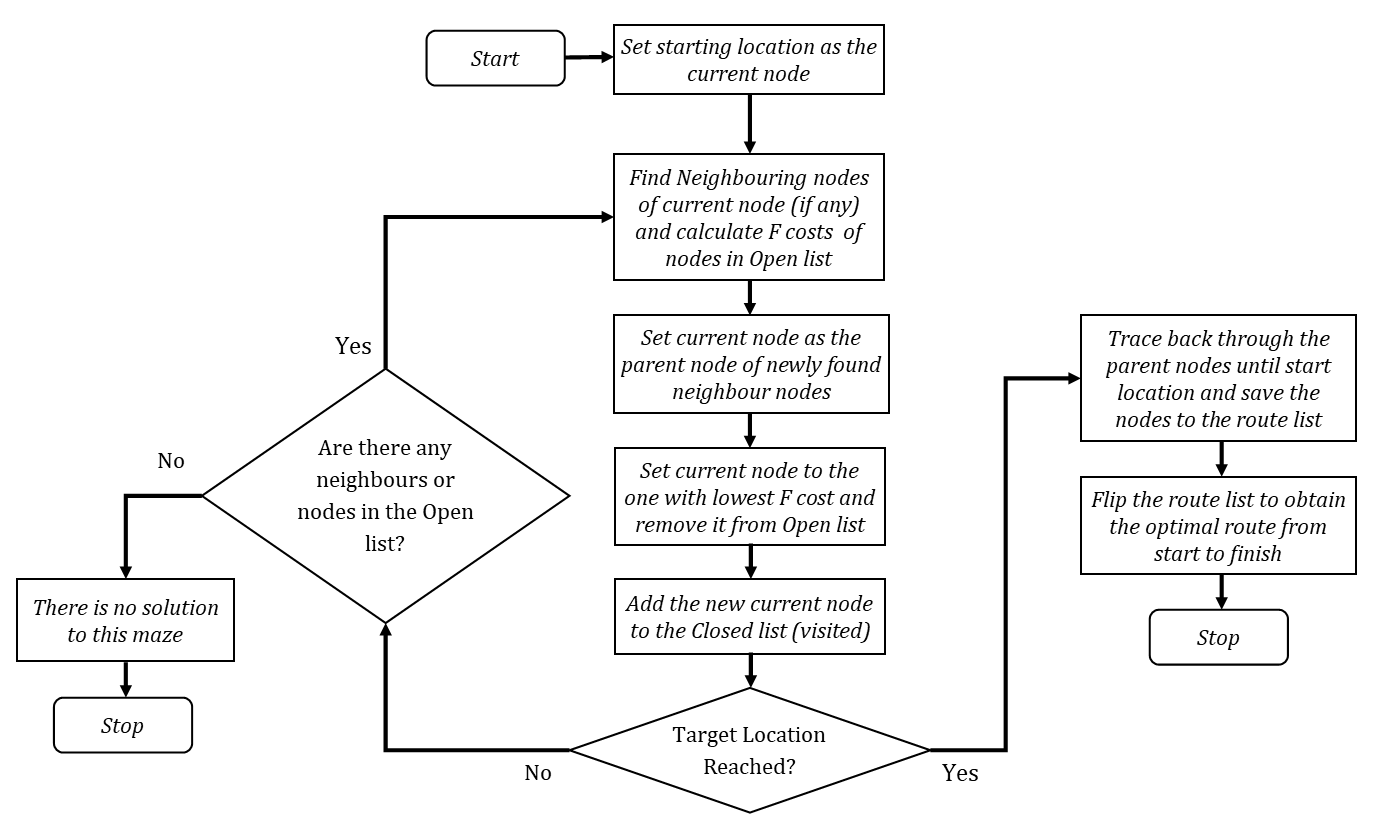
\includegraphics[width=0.5\textwidth]{a_star_diagram}}
\caption{A* Algorithm Flowchart}
\label{fig:astar}
\end{figure}

\begin{figure}[!h]
\centerline{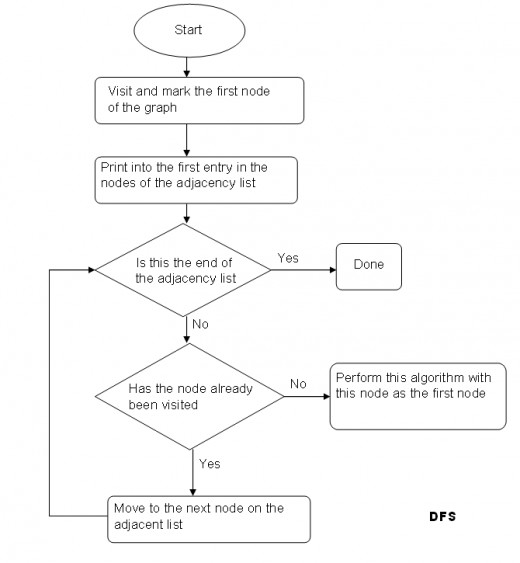
\includegraphics[width=0.5\textwidth]{dfs_diagram}}
\caption{DFS Algorithm Flowchart}
\label{fig:dfs}
\end{figure}

\begin{figure}[!h]
\centerline{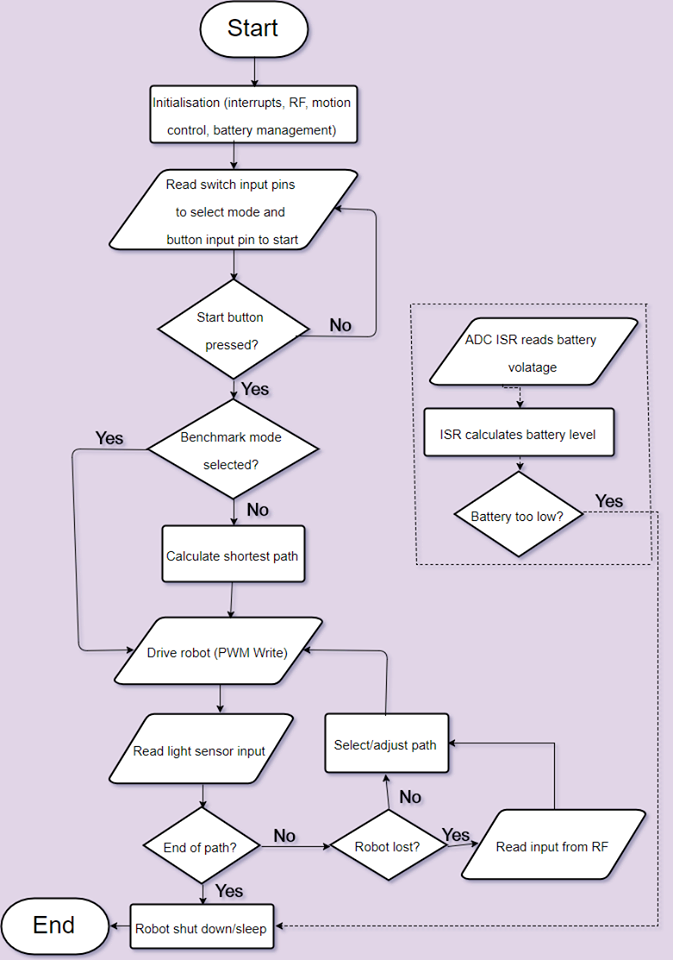
\includegraphics[width=0.5\textwidth]{software_flowchart}}
\caption{Overall Software Flowchart}
\label{fig:overallsoftchar}
\end{figure}

\vfill

\clearpage

\section{Appendix B: Sensors}

\subsection{Sensor Layout}

The circuit used to process the sensor data and the layout used to place the sensors on the PCB were essential to ensuring the success of the project. This appendix covers these two components of the project in greater detail.

\begin{figure}[!h]
\centerline{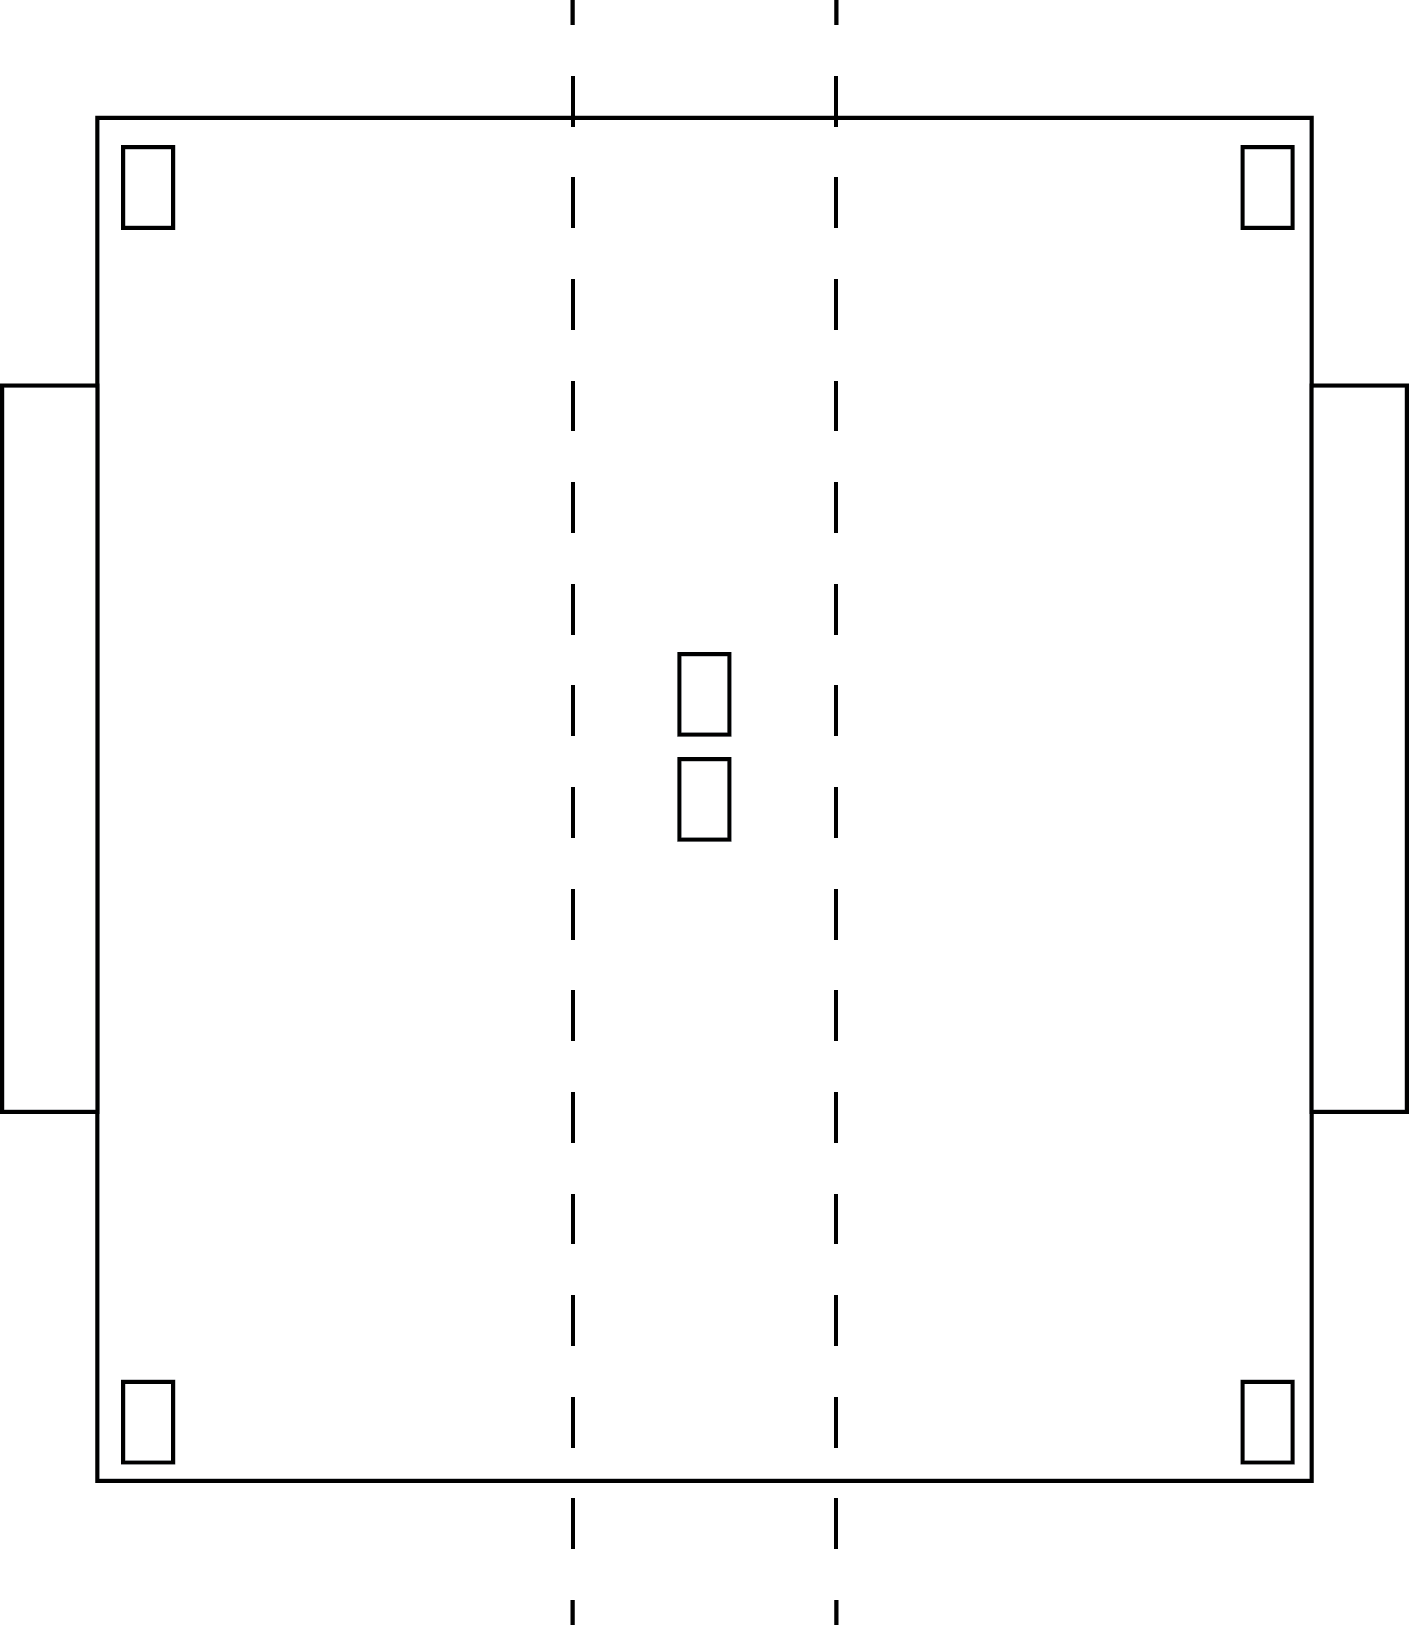
\includegraphics[width=0.5\textwidth]{outer_edge_sensor}}
\caption{Outer Edge Sensor Layout}
\label{fig:outer_edge_sensor}
\end{figure}

Various layouts for the sensors were considered during the course of the project, these are outlined below. The first sensor layout to considered was the Outer Edge Sensor layout, shown in \Cref{fig:outer_edge_sensor}. This is a sensor arrangement with all the sensors at the extreme ends of the board. This allows us to capture a wider picture of where the robot is. This will be able to to detect intersections in advance of arriving at them. This layout also doesn't have the capability to closely track a line.

Another layout that was considered was the Circular Sensor Arrangement as in \Cref{fig:circular_sensor}. This layout would not be able to detect that the robot is deviating off the line, until the robot has fully left the line. This would make it harder to keep the oscillations shallow and follow the line reasonably straight. This layout would also introduce a delay while detecting intersections, as the side sensors are further back from the edge. This means there might not be enough notice to brake in time.

The next sensor considered was in a parabola shape (\Cref{fig:parabola_sensor}). In this arrangement the robot would be able to very closely follow the line applying only small corrections to ensure that the robot follows the line.

\begin{figure}[!h]
\centerline{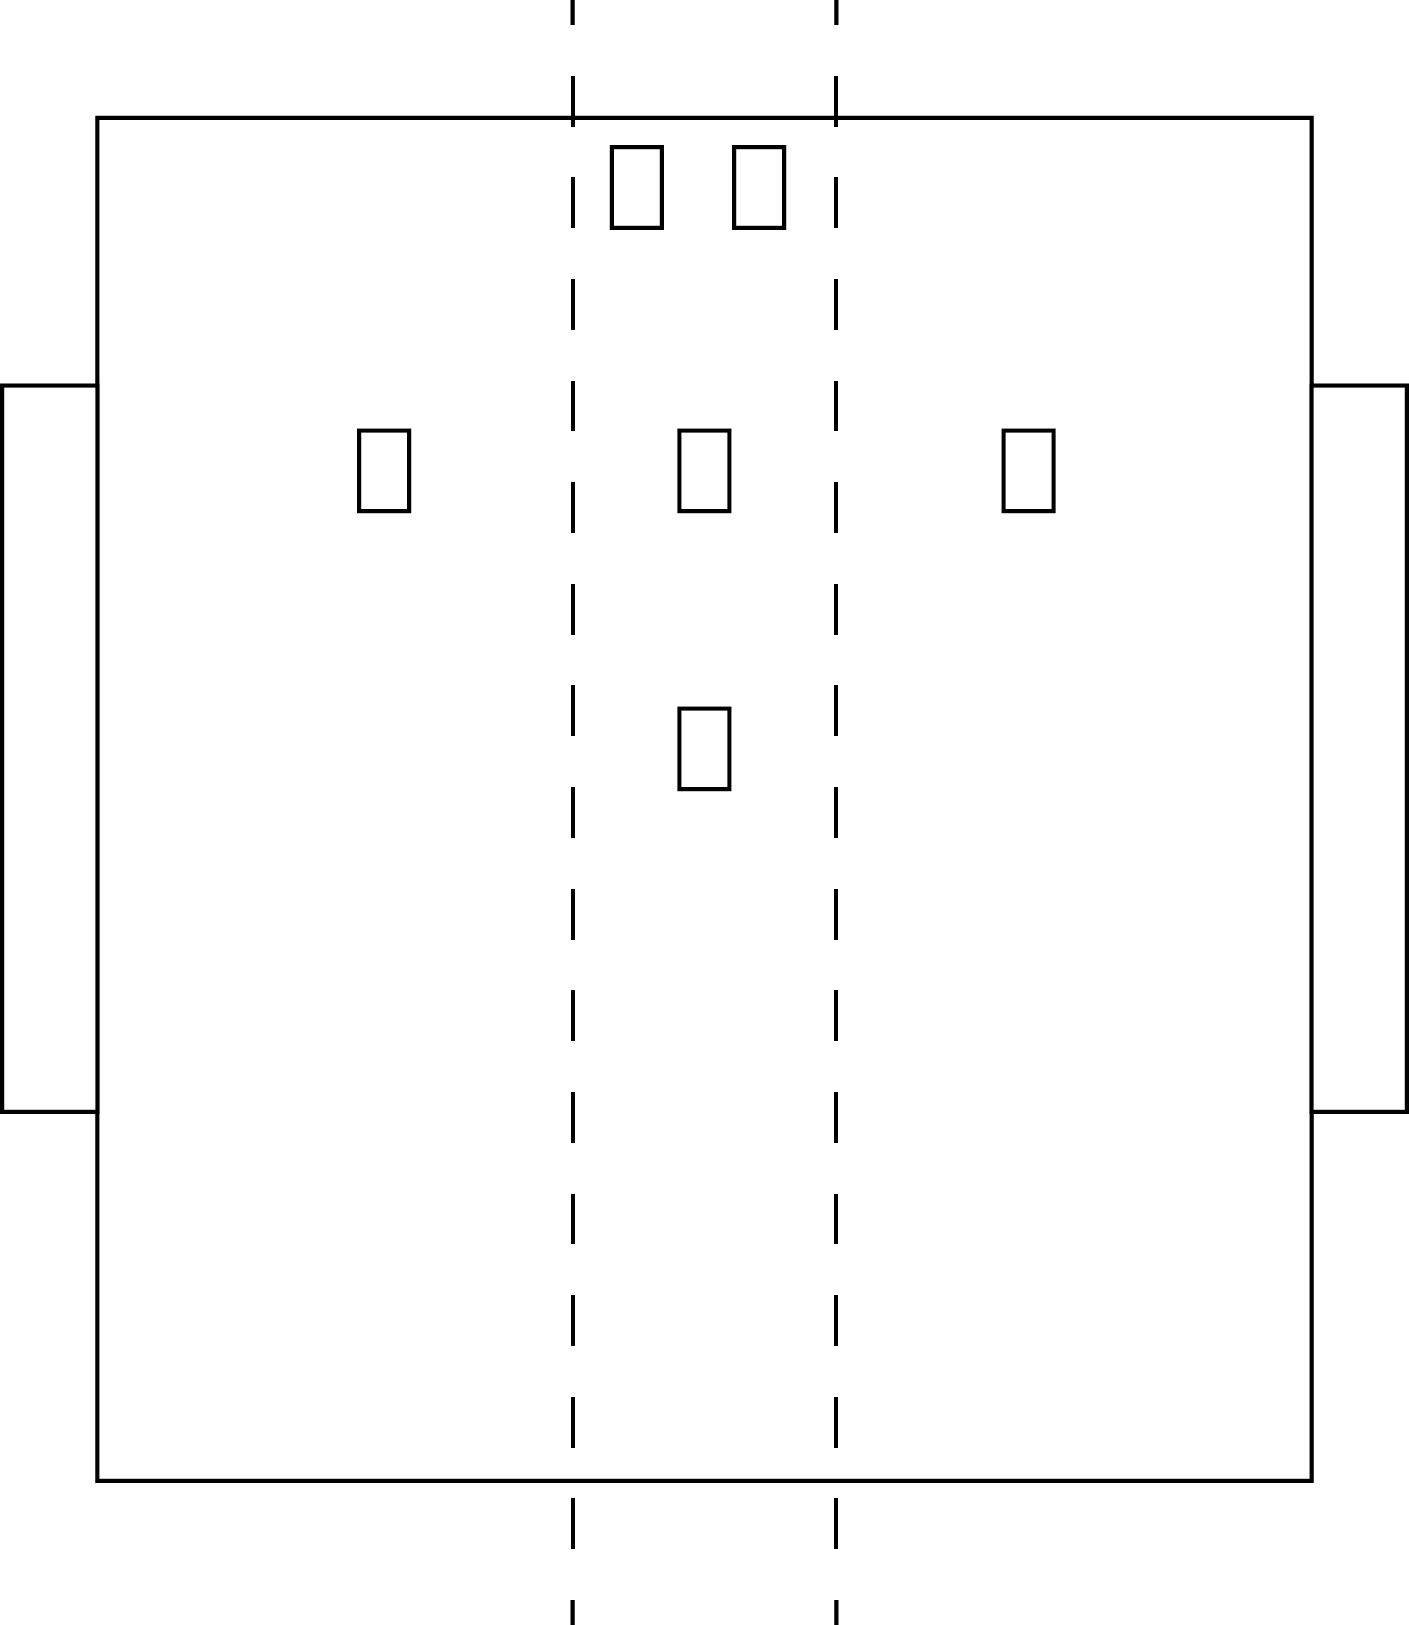
\includegraphics[width=0.5\textwidth]{circular_sensor}}
\caption{Circular Sensor Layout}
\label{fig:circular_sensor}
\end{figure}

\begin{figure}[!h]
\centerline{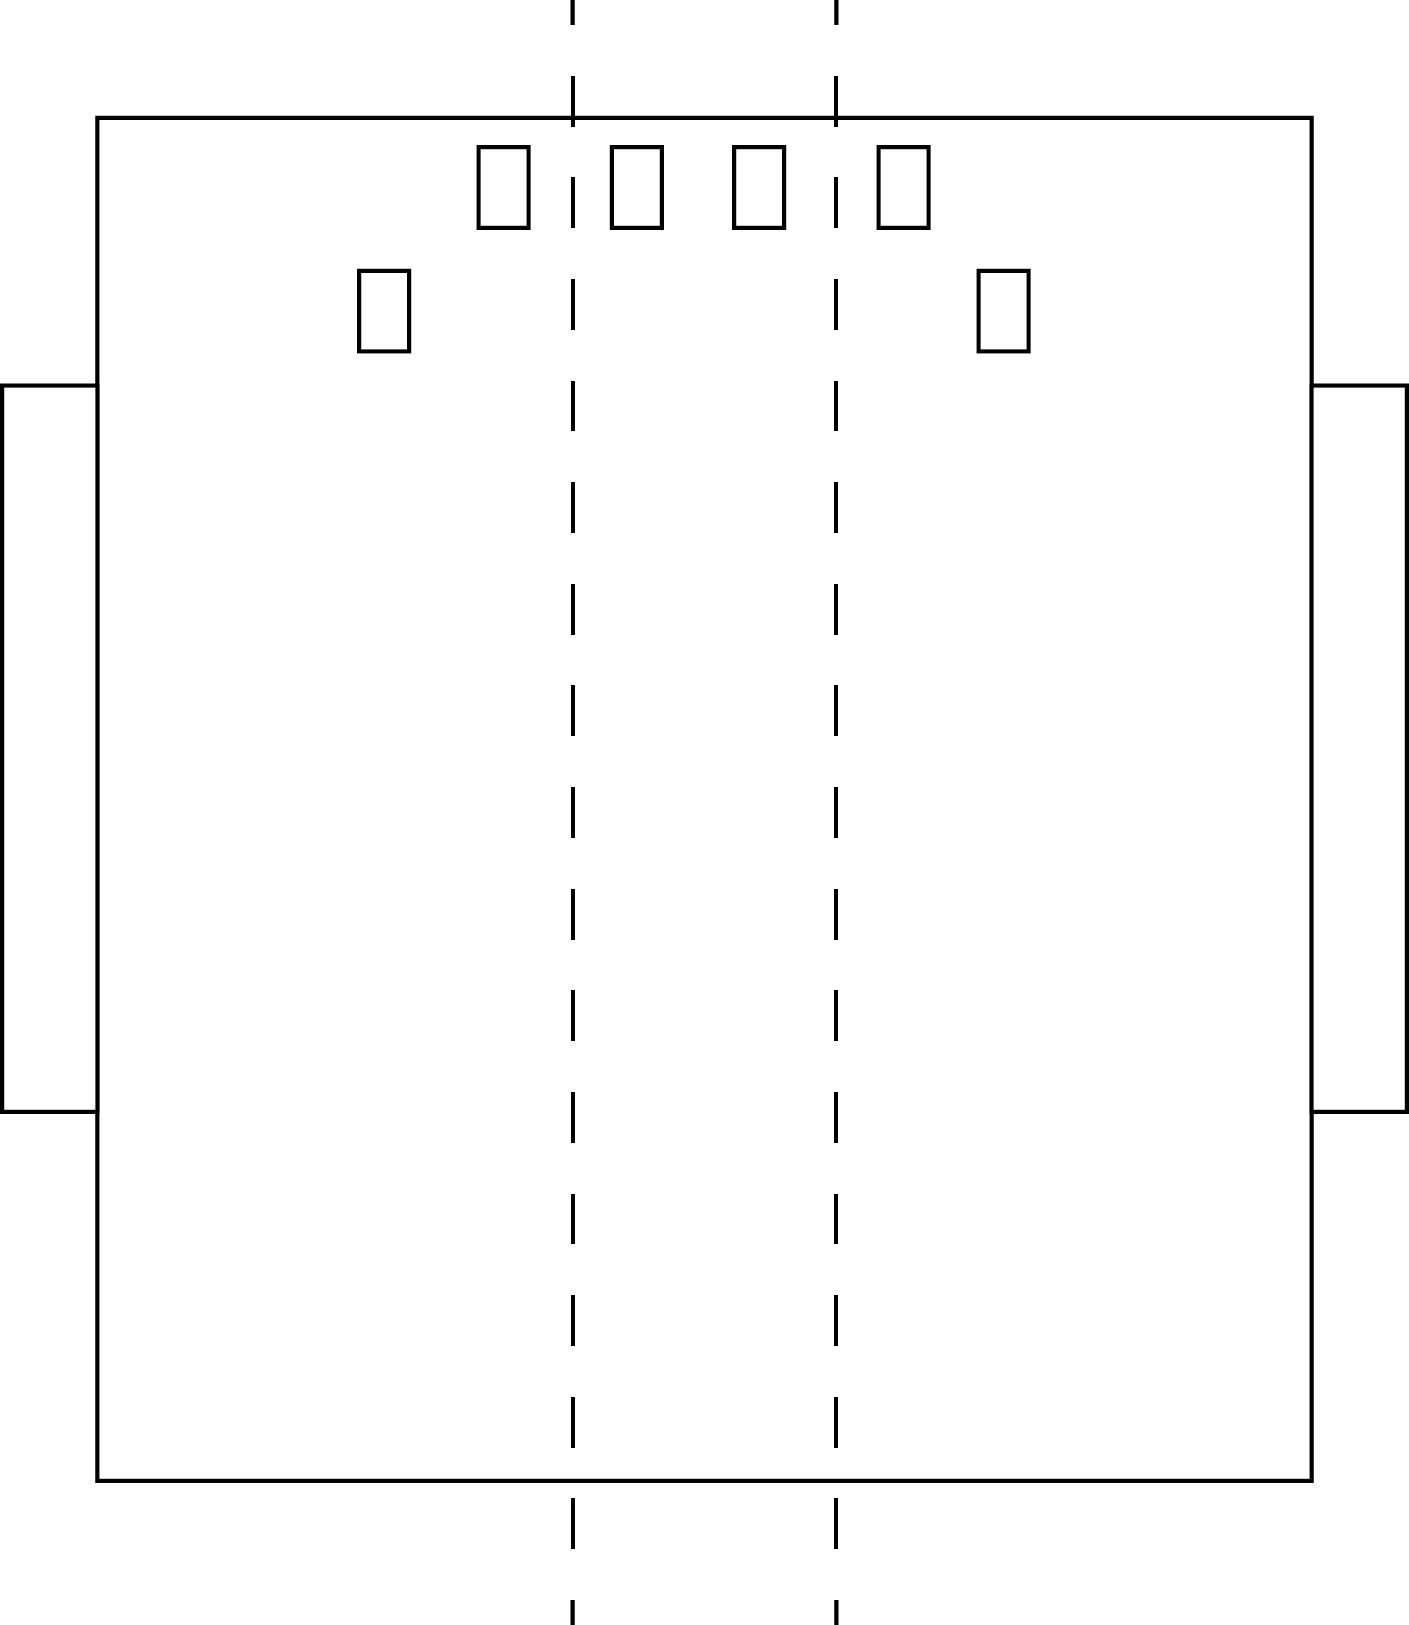
\includegraphics[width=0.5\textwidth]{parabola_sensor}}
\caption{Parabolla Sensor Layout}
\label{fig:parabola_sensor}
\end{figure}

Another arrangement that was considered was the straight line sensor arrangement (\Cref{fig:the_straight_line_sensor}). This arrangement was a slight improvement over the parabola layout. This was far easier to design and assemble as the sensors just need to be placed in an equidistant manner in a straight line. This layout will allow the robot to calculate the deviation from the line and apply accurate corrections to return to the line.

The modified straight line sensor  (\Cref{fig:modified_straight_line_sensor}) was what was used in the final design. This was chosen with the aim of being able to see detect how far off the line the robot had travelled before turning, whilst also providing all the benefits of the straight line configuration.

\begin{figure}[!h]
\centerline{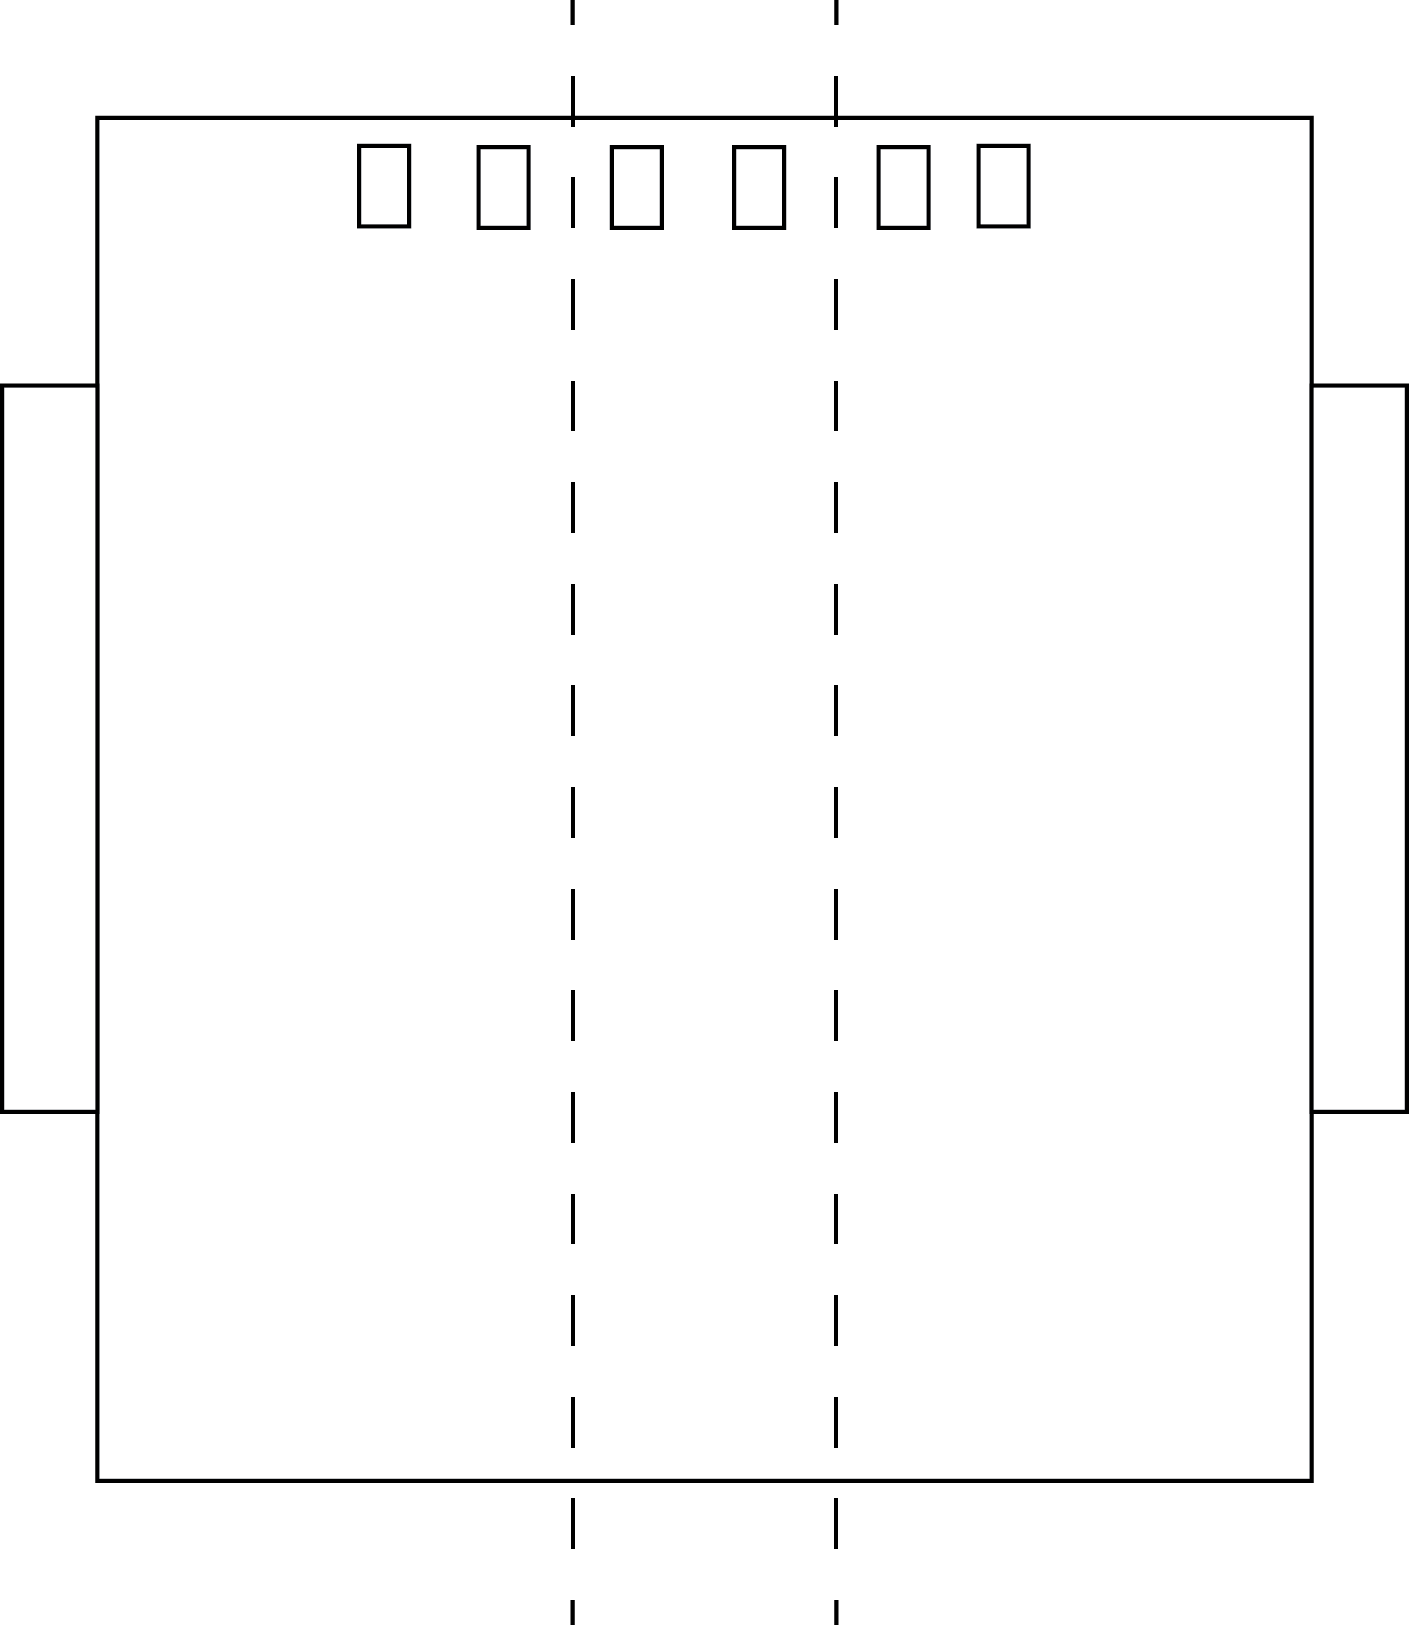
\includegraphics[width=0.5\textwidth]{the_straight_line_sensor}}
\caption{The Straight Line Sensor Layout}
\label{fig:the_straight_line_sensor}
\end{figure}

\begin{figure}[!h]
\centerline{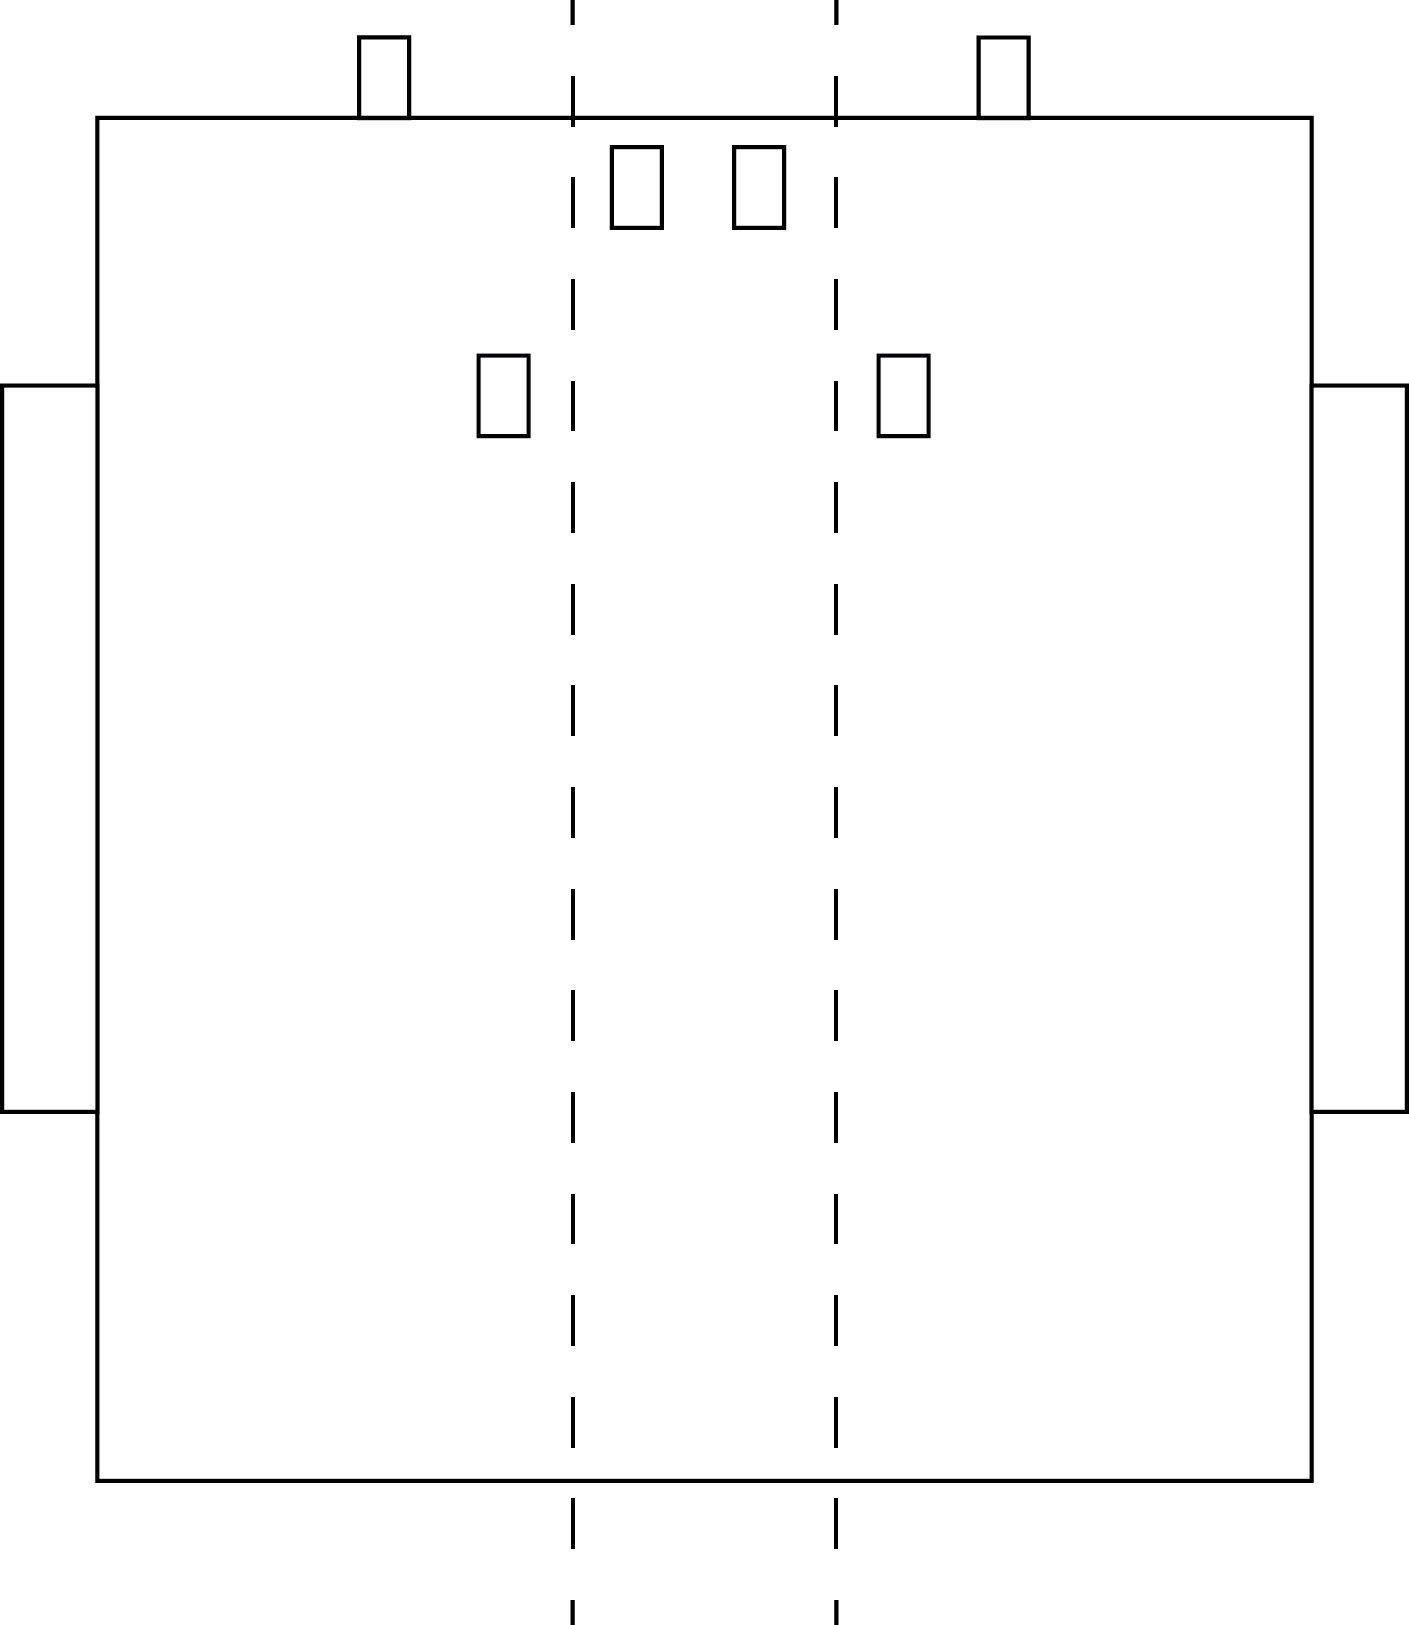
\includegraphics[width=0.5\textwidth]{modified_straight_line_sensor}}
\caption{The Modified Line Sensor Layout}
\label{fig:modified_straight_line_sensor}
\end{figure}

\clearpage

\subsection{Sensor Processing Circuit}

\begin{table}[htbp]
  \centering
  \caption{Summary of Sensor Output Signal}
    \begin{tabular}{rrr}
          & \multicolumn{1}{l}{\textbf{BLACK LIGHT}} & \multicolumn{1}{l}{\textbf{WHITE LIGHT}} \\
          &       &  \\
    \multicolumn{1}{l}{MAX} & 2.0650 & 2.2180 \\
    \multicolumn{1}{l}{MIN} & 1.9060 & 0.4679 \\
    \multicolumn{1}{l}{PK-PK} & 0.1590 & 1.7501 \\
    \multicolumn{1}{l}{\textbf{AVG}} & \textbf{1.9913} & \textbf{1.4281} \\
    \multicolumn{1}{l}{RMS} & 1.9918 & 1.5475 \\
    \multicolumn{1}{l}{\textbf{Amp}} & \textbf{0.0795} & \textbf{0.8751} \\
          &       &  \\
    \end{tabular}%
  \label{tab:addlabel}%
\end{table}%

The sensor circuit used in this project consisted of four components; a RC High pass filter, gain stage, Peak detector \& Schmitt trigger. The first stage in the processing circuit was a RC high pass filter. This was a first order filter with a cut-off frequency of 106.1Hz. This cut off frequency was chosen as this was between the signal we wanted (120Hz) and the main source of noise (100Hz). The resulting signal had removed most of the noise and was centred around 0V.

\begin{figure}[!h]
\centerline{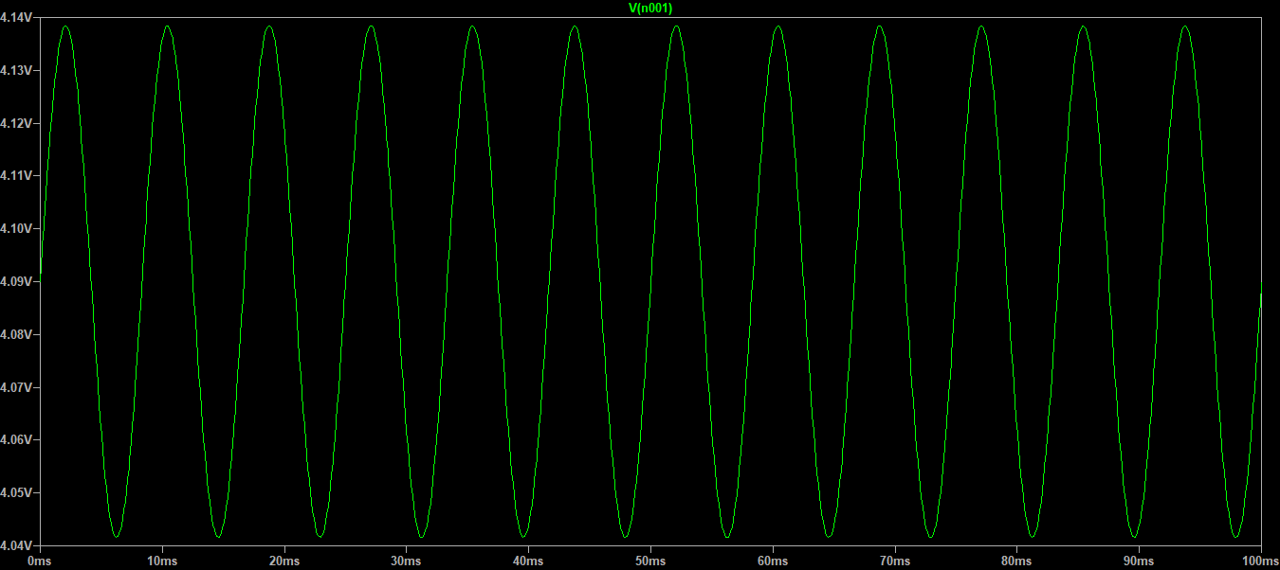
\includegraphics[width=0.5\textwidth]{stage_1}}
\caption{Signal from Phototransistor}
\label{fig:stage1}
\end{figure}

\begin{figure}[!h]
\centerline{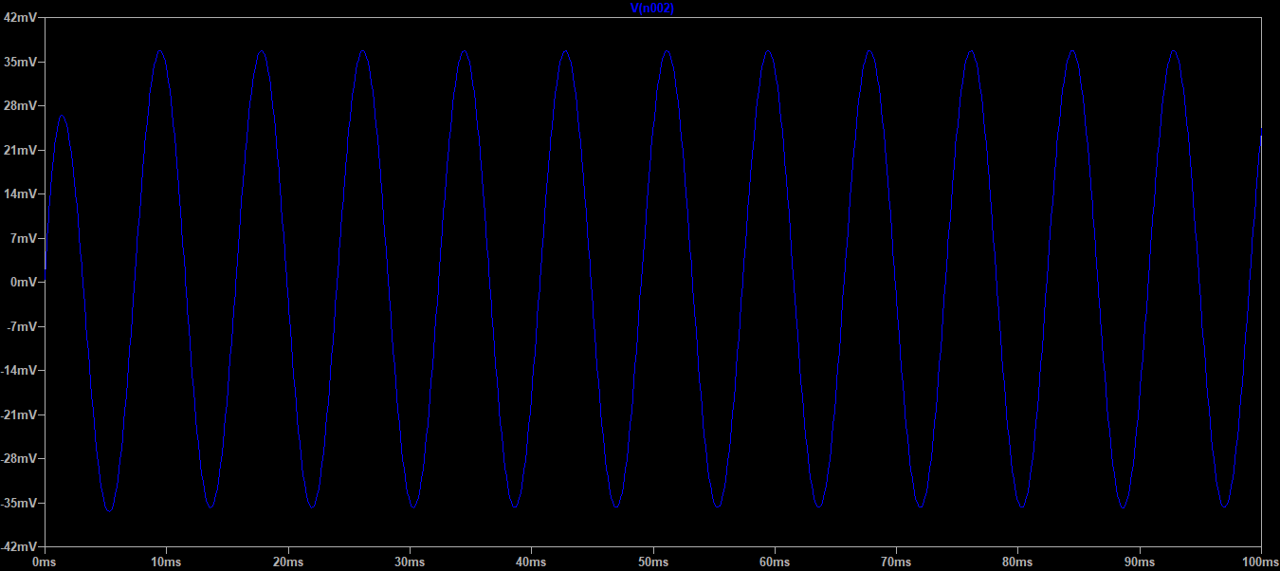
\includegraphics[width=0.5\textwidth]{stage_2}}
\caption{After the RC High pass filter}
\label{fig:stage2}
\end{figure}

The resulting signal from after the RC high pass filter was quite small in amplitude and needed to be amplified before it could be further processed. A 20x gain stage was used in a non-inverting op-amp configuration. The op-amp used was supplied from a single supply and therefore the bottom half of the signal was discarded, this was not necessary for our final output and therefore is not a concern.

\begin{figure}[!h]
\centerline{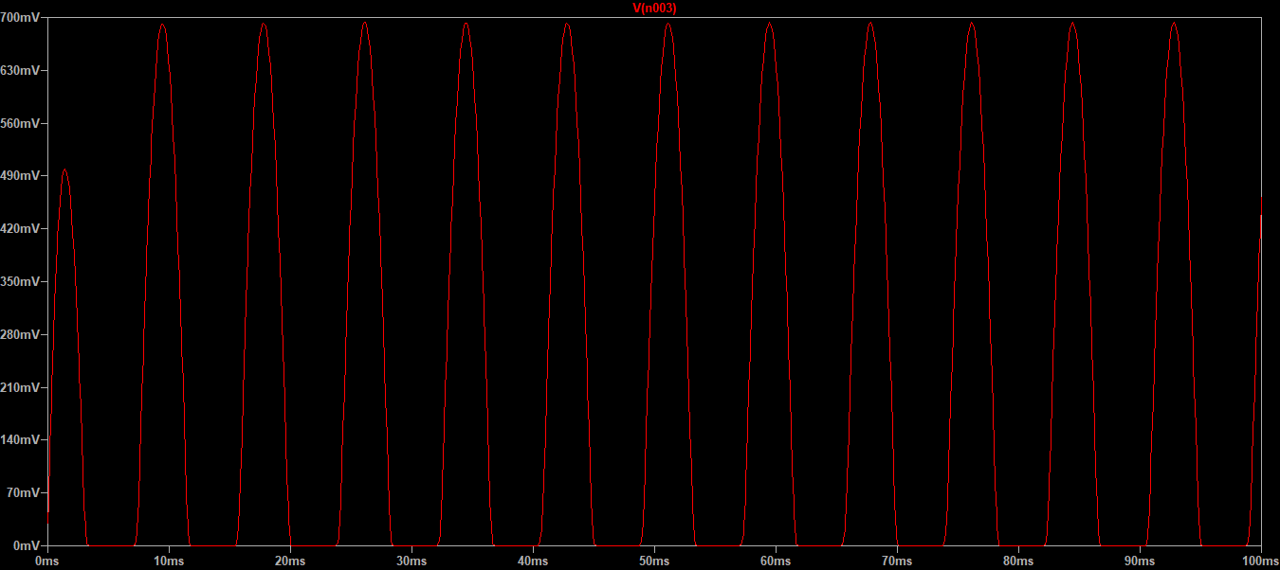
\includegraphics[width=0.5\textwidth]{stage_3}}
\caption{Signal after the Gain stage}
\label{fig:stage3}
\end{figure}

The next stage of the circuit is a peak detector circuit which allowed for quick capture of just the peak amplitude of the signal and discard all other information. This was used as the peak amplitude was the main characteristic that differentiated the black and white lights and therefore was enough for this project. Finally a Schmitt trigger circuit was used with a carefully selected cut-off of 2.67V to produce a digital output of either a HIGH or LOW to represent whether the light sensor was currently on or off the line.

\begin{figure}[!h]
\centerline{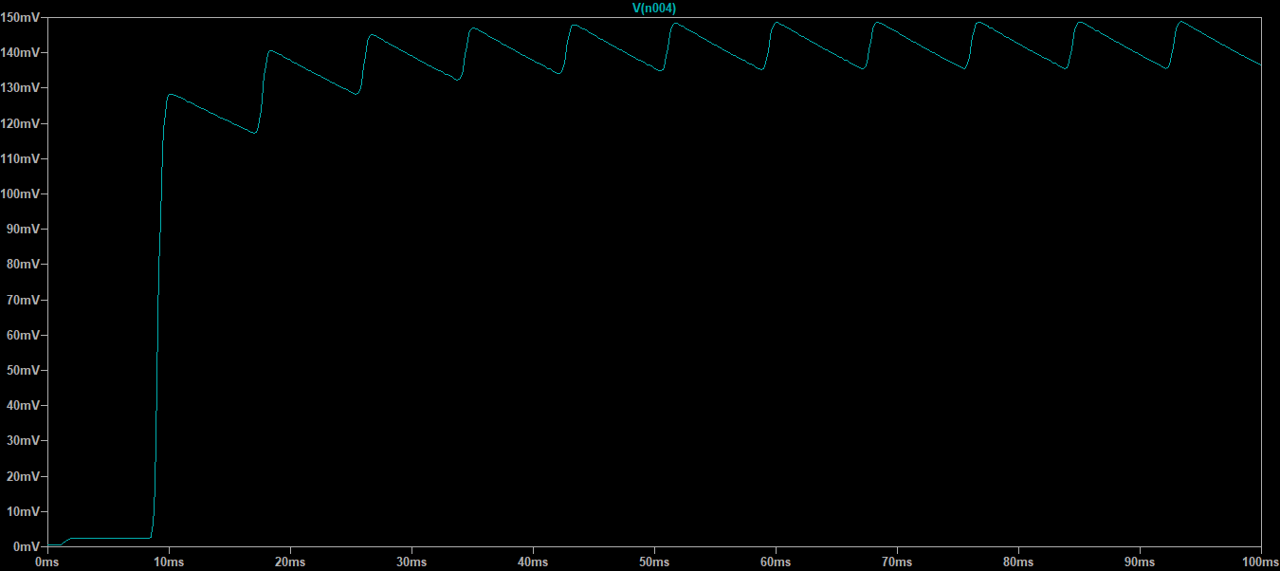
\includegraphics[width=0.5\textwidth]{stage_4}}
\caption{Signal after peak detector circuit}
\label{fig:stage4}
\end{figure}

\begin{figure}[!h]
\centerline{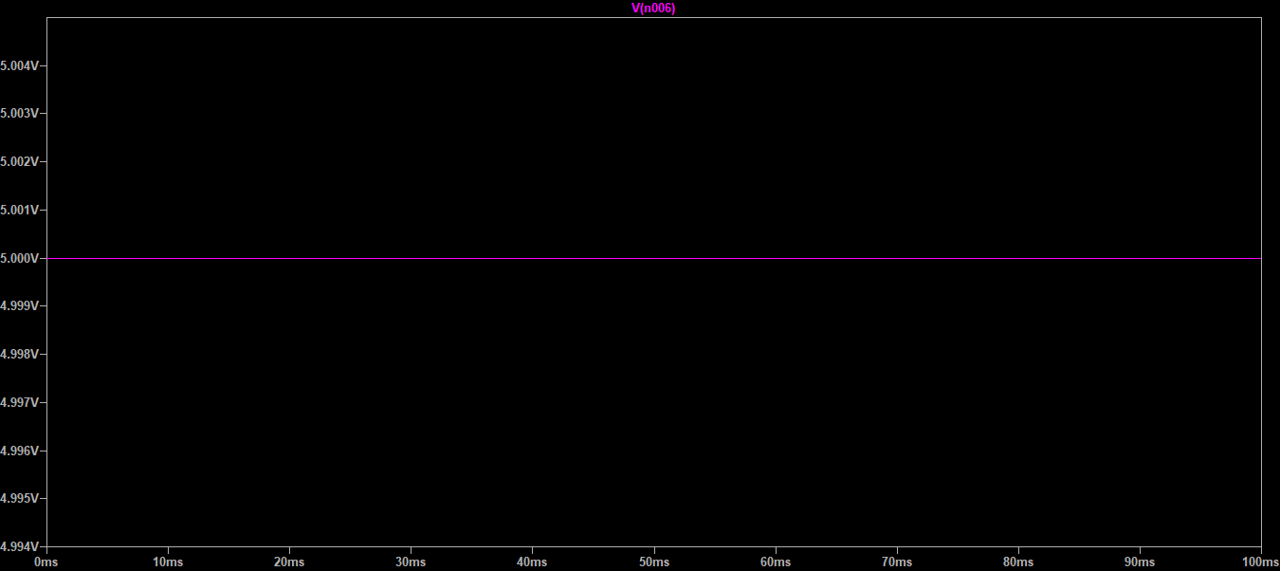
\includegraphics[width=0.5\textwidth]{stage_5}}
\caption{Final signal send to PSoC}
\label{fig:stage5}
\end{figure}

\end{document}